\documentclass[conference]{IEEEtran}
\IEEEoverridecommandlockouts
\usepackage[nocompress]{cite}
\usepackage{amsmath,amssymb,amsfonts}
\usepackage{graphicx}
\usepackage{textcomp}
\usepackage{booktabs}
\usepackage{url}
\usepackage{multirow}

\begin{document}

\title{Confidently Wrong: Silent Failures of Classical and Learned Feature Matching for GPS-Denied UAV Localization}

\author{
\IEEEauthorblockN{Kana Am\'ed\'ee}
\IEEEauthorblockA{Independent Researcher \\
Bujumbura, Burundi \\
kanaamedee00@gmail.com \\
ORCID 0009-0009-9620-6399 \\
Code: github.com/kanaamedee11/confidently-wrong-skygaze}
}

\maketitle

\par\noindent{\small\bfseries\itshape Abstract. }{\small\bfseries @@ABSTRACT@@\par}
\vspace{0.6\baselineskip}
\par\noindent{\small\bfseries\itshape Keywords. }{\small\bfseries visual localization, UAV navigation, GPS-denied navigation, feature matching, SuperGlue, failure analysis, selective prediction\par}

\section{Introduction}

Autonomous UAVs increasingly operate where GPS cannot be trusted: urban canyons that occlude satellites, deliberate jamming, and remote regions with degraded correction signals. When GPS is lost, a UAV usually still has an onboard camera and a stored georeferenced reference image of the area it expects to overfly, such as a satellite tile or an orthophoto. \emph{Visual localization} uses these two to recover position without any satellite signal: the live frame (the \emph{query}) is matched against the reference, and the estimated geometric relation gives the vehicle's location.

The problem is studied under several names, including cross-view geo-localization, terrain-referenced navigation, and GPS-denied visual localization \cite{zheng2020university,zhu2021vigor,goforth2019gps}. A recurring design choice is how the query and reference are matched: with hand-crafted local features such as SIFT \cite{lowe2004distinctive} and ORB \cite{rublee2011orb}, or with a learned matcher such as SuperPoint and SuperGlue \cite{detone2018superpoint,sarlin2020superglue}. Comparisons between them are usually reported as accuracy on a benchmark. For a navigation system, a second question matters at least as much: \emph{when a matcher fails, does the system know?} A matcher that declines to answer is an inconvenience; a matcher that confidently returns a wrong position is a hazard, because the downstream controller has no reason to distrust it.

This paper builds a small, fully reproducible harness to study exactly that, and reports six contributions.
\begin{enumerate}
\item \textbf{A modular pipeline and evaluation harness.} SkyGaze runs SIFT, ORB and SuperPoint+SuperGlue behind one interface with identical geometric verification, so differences are attributable to the matching stage.
\item \textbf{An outcome taxonomy.} Every trial is classified as \emph{accurate}, \emph{detected failure} (no homography), or \emph{silent failure} (a wrong homography returned as a success). Counting any returned homography as success, as is common, hides the third class entirely.
\item \textbf{A controlled study with exact ground truth} over in-plane rotation and six further degradation axes (scale, perspective, noise, blur, occlusion, appearance), with @@NTRIALS@@ trials in total and confidence intervals.
\item \textbf{A sharp failure mode of the learned matcher, and a cheap remedy.} SuperGlue is the most accurate method up to $45^\circ$ of rotation but collapses within the next $15^\circ$, returning wrong homographies. Evaluating four rotated copies of the query and keeping the hypothesis with the most RANSAC inliers removes the failure at four times the cost.
\item \textbf{A confidence-gate analysis.} We show how well the RANSAC inlier count separates correct from silently wrong localizations, as a risk-coverage trade-off \cite{elyaniv2010foundations}.
\item \textbf{A real-data check.} On 32 held-out frames of a real UAV-VisLoc flight matched against its real satellite map, the same three outcomes are measured in metres (Section~\ref{sec:real}).
\end{enumerate}
We are explicit about scope: the controlled study is synthetic, with queries that are transformed crops of the reference, so its absolute numbers do not transfer to real drone imagery. The real-data check uses one flight, one satellite map and 32 frames, so it tests whether the failure structure carries over and does not establish rates for UAV-VisLoc as a whole.

\section{Related Work}

\textbf{Cross-view geo-localization.} University-1652 \cite{zheng2020university} frames drone, satellite and ground views of the same place as a multi-view retrieval problem, and VIGOR \cite{zhu2021vigor} moves beyond one-to-one retrieval toward finer, city-scale localization. Goforth and Lucey \cite{goforth2019gps} address GPS-denied UAV localization directly against pre-existing satellite imagery with learned features. UAV-VisLoc \cite{xu2024uavvisloc} pairs 6{,}742 real drone images with 11 georeferenced satellite maps and per-image ground truth, and is the benchmark we target for real-data evaluation.

\textbf{Local feature matching.} SIFT \cite{lowe2004distinctive} and ORB \cite{rublee2011orb} remain standard baselines because they are fast, interpretable and need no training data; both are followed by geometric verification, typically RANSAC \cite{fischler1981random}. SuperPoint \cite{detone2018superpoint} learns keypoints and descriptors, and SuperGlue \cite{sarlin2020superglue} learns the matching itself with attention over keypoint sets; its outdoor weights are trained on MegaDepth \cite{li2018megadepth}. Detector-free LoFTR \cite{sun2021loftr} and the faster LightGlue \cite{lindenberger2023lightglue} are more recent; we do not evaluate them here (Section~\ref{sec:limits}).

\textbf{Knowing when to abstain.} Selective prediction studies the trade-off between the fraction of inputs a model answers (coverage) and its error on the answered ones (risk) \cite{elyaniv2010foundations}. We apply this view to localization: a geometric-verification score (the RANSAC inlier count) is the confidence signal, and a threshold on it is the gate.

\section{Method}

\subsection{Problem and pipeline}
Given a reference image $R$ and a query $Q$, the goal is a homography $H$ mapping query pixels to reference pixels, from which the vehicle position, taken as the image of the query centre $c_Q$, is $\hat{p}=H c_Q$. Fig.~\ref{fig:pipeline} shows the pipeline. Keypoints are extracted and matched, RANSAC \cite{fischler1981random} (5.0\,px reprojection threshold, shared by all matchers) estimates $H$ and an inlier set, and a confidence gate decides whether to accept the result.

\begin{figure*}[t]
\centering
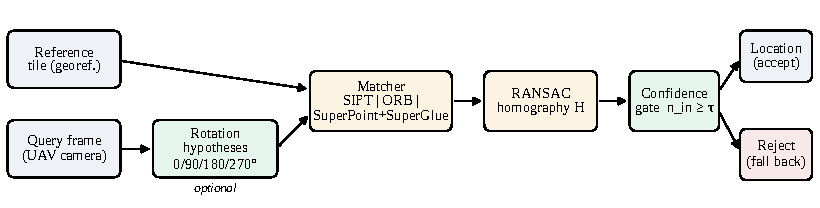
\includegraphics[width=0.96\textwidth]{figures/fig_pipeline_v2.pdf}
\caption{SkyGaze pipeline. The matcher is swappable behind one interface. Two stages are optional additions studied here: rotation hypotheses in front of the matcher, and a confidence gate on the RANSAC inlier count after it.}
\label{fig:pipeline}
\end{figure*}

\subsection{Matchers}
\textbf{SIFT} \cite{lowe2004distinctive}: brute-force L2 matching with Lowe's ratio test at 0.75. \textbf{ORB} \cite{rublee2011orb}: up to 4000 features, Hamming matching with the same ratio test. \textbf{SuperGlue} \cite{sarlin2020superglue}: SuperPoint keypoints (at most 1024, threshold 0.005) matched with the pretrained outdoor weights and a match threshold of 0.2. No matcher is tuned on the benchmark.

\subsection{Rotation hypotheses}
Because the cliff reported in Section~\ref{sec:rot} is a function of in-plane rotation, we add a test-time variant, \emph{SuperGlue + rot.\ hyp.}: the query is rotated by $0^\circ$, $90^\circ$, $180^\circ$ and $270^\circ$, each version is matched against the reference, and the hypothesis with the most RANSAC inliers is kept, with its homography composed with the known rotation. Any residual rotation is at most $45^\circ$, inside the range where plain SuperGlue is reliable. The cost is four forward passes.

\subsection{Outcomes, metrics and the confidence gate}
The localization error is $e=\lVert H c_Q - p^{*}\rVert$, in pixels of the $800\times800$ reference, where $p^{*}$ is the exact ground-truth position. A trial is \emph{accurate} if a homography is returned and $e\le\tau$ with $\tau=10$\,px (1.25\% of the reference width); a \emph{silent failure} if a homography is returned with $e>\tau$; and a \emph{detected failure} if none is returned. We report the accurate rate with 95\% Wilson intervals \cite{wilson1927probable}, and the median error among accurate trials.

The gate accepts a result when its RANSAC inlier count is at least $\tau_n$. Sweeping $\tau_n$ gives a risk-coverage curve: coverage is the fraction of all trials accepted, and risk is the fraction of accepted trials that are wrong. We also report the AUROC with which the inlier count separates accurate from non-accurate trials.

\section{Experimental Protocol}

\textbf{Data.} Three procedurally generated $800\times800$ references (fields, a road network and buildings on textured ground, seeds 0 to 2) provide scenes with known structure and no third-party imagery. A query is a $280\times280$ sub-region at a random offset, warped by a known transform, so the ground-truth homography is exact. To test dependence on texture statistics we repeat the rotation sweep on a second domain: a $2\times2$ mosaic of four photographic ground textures (gravel, grass, brick, rotated gravel) from the scikit-image sample data. Fig.~\ref{fig:data} shows the references and one example query per degradation.

\begin{figure*}[t]
\centering
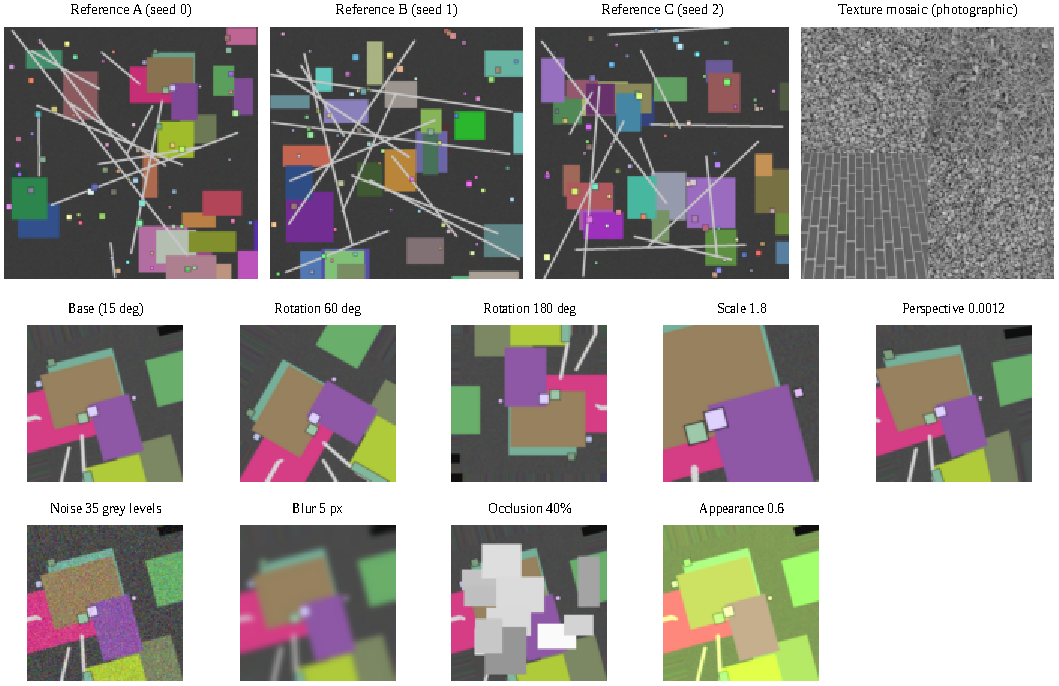
\includegraphics[width=0.86\textwidth]{figures/fig_data_v2.pdf}
\caption{Test imagery. Top: the three generated $800\times800$ reference scenes and the photographic texture mosaic. Below: example $280\times280$ queries cut from Reference A at one location, each showing one degradation at the level named in its title (the base condition is $15^\circ$ rotation, scale 0.9).}
\label{fig:data}
\end{figure*}

\textbf{Degradation axes.} Rotation is swept alone at scale 0.9. The six other axes are swept one at a time around a base condition (rotation $15^\circ$, scale 0.9, brightness $+15$, blur $\sigma=0.8$\,px): scale (query zoom) in $\{0.5, 0.7, 0.9, 1.3, 1.8\}$; a perspective coefficient in $\{0, 2, 4, 8, 12\}\times10^{-4}$ (at the highest value the apparent scale changes by about $\pm17\%$ across the frame edge); additive Gaussian noise $\sigma\in\{0,10,20,35\}$ grey levels; blur $\sigma\in\{0.8,2,3.5,5\}$\,px; occlusion by opaque rectangles covering $\{0,20,40,60\}\%$ of the query; and an appearance gap, a random per-channel gain and global gamma change of strength $\{0,0.2,0.4,0.6\}$.

\textbf{Trial counts.} @@TRIALCOUNTS@@ Every matcher sees the same references and seeds. All runs are on CPU (2 vCPU); SuperGlue uses the public pretrained outdoor weights. Code, trial-level results and the figure scripts are included with the project.

\textbf{Measurement note.} The pipeline's original localization estimate was the mean of the four projected query corners. This equals the projection of the query centre only for similarity transforms; under a perspective component it does not, and would have reported a spurious failure on the perspective axis. All errors here use $H c_Q$.

\section{Results}

@@RESULTS@@

\section{Discussion and Limitations}
\label{sec:limits}

@@DISCUSSION@@

\section{Conclusion}

@@CONCLUSION@@

\bibliographystyle{IEEEtran}
\bibliography{references}

\end{document}
